\chapter{Gamma-Ray Astronomy in the Context of Astroparticle Physics}

The last two decades have been revolutionary for astronomy.
For the first time, observations are routinely carried out over the whole
electromagnetic spectrum from radio wavelengths to very high energy gamma radiation.
Joining in, first observations of gravitational waves in 2015~\cite{ligo-bbm}
and a first hint of neutrinos~\cite{txs} from a gamma-ray source bring us to the verge of true multi-messenger astronomy. 
Only provided by the full picture of the universe as delivered by photons
over the whole electromagnetic spectrum, neutrinos and gravitational waves,
can we hope to understand the processes governing the high energy universe,
which produces particles at energies out of reach for particle accelerators on Earth.
The field of astroparticle physics combines techniques, methods and theory from high energy
particle physics to study the universe through these high energy cosmic messengers 
reaching Earth.

In the following sections, I will give an introduction into the general field
of astroparticle physics in \autoref{sec:messengers},
especially gamma-ray astronomy, and the crucial role it plays in understanding our universe.
I will present the currently operating and planned gamma-ray observatories in \autoref{sec:telescopes},
the most common sources of gamma radiation in \autoref{sec:sources}
and the key questions that are currently pursued in \autoref{sec:science}.
I will discuss charged cosmic rays, mainly focussing on the role they play in gamma-ray astronomy in \autoref{sec:cosmic-rays}.

After the general introduction into the field, I will introduce the \gls{fact},
the instrument used to perform my studies, in \autoref{chp:fact}, its mission and
properties important for the context of my work.

Due to the non-existence of artificial sources for calibration, 
high-energy astrophysics experiments must heavily rely on simulations.
This is necessary for tuning of detector parameters,
estimating performance and creating datasets with known physical properties
to be able to reconstruct these properties for recorded events.
The simulations performed for this work are detailed in \autoref{chp:simulation}.

\hyperref[chp:preprocessing]{Chapter~}\ref{chp:preprocessing} will present the data analysis techniques used
to make sense of the raw data and how the vast amounts of data are reduced
to a more manageable size while keeping most of the relevant information
via the use of few but descriptive properties.

From these features, estimators for the physical properties of the 
detected particles are created through the means
of statistical learning. 
This is the topic of \autoref{chp:reconstruction}.

The first part of this thesis is concluded with the presentation
of the sensitivity and  instrument response functions
of the combined system of telescope and data analysis in \autoref{chp:performance}.
These will be evaluated both on simulated and observed data where possible.
Finally, estimating the energy spectrum of the Crab Nebula will be the topic of \autoref{chp:spectrum}.

In a smaller second part, the effort put in to make \gls{fact} a robotically operating telescope,
observing on its own nearly without the need of human intervention or supervision,
is presented in \autoref{chp:shifthelper}.

At the very end, synopsis and prospects of further work is provided in \autoref{chp:outlook}.

\section{Cosmic Messengers}\label{sec:messengers}

Information about the universe is reaching Earth through multiple kinds of radiation and stable particles.
Each kind has its own challenges in detecting the messengers and extracting the contained information.
The different messengers are also unique in the kind of information they are able to convey.

Since the dawn of humanity, people have looked into the sky and observed
it in the visible spectrum, first with naked eyes then with ever larger and
better telescopes.
Radio observatories enabled a first glimpse at the non-thermal universe and observing the thermal remnants of the Big Bang.
The advent of space flight made telescopes not hindered by absorption of light
in Earth's atmosphere, light pollution and adverse weather conditions possible.
Together with photographic plates and electronic photodetectors,
this opened up observations in wavelengths not accessible before,
including the far infrared, X-rays and gamma rays.
Finally, the \gls{iact} technique allows for observations of gamma ray sources at energies
larger than \SI{100}{\GeV}.
Observations of gamma rays will be discussed in detail in \autoref{sec:telescopes}.

Earth is constantly bombarded by high energy charged particles, cosmic rays.
These particles reach energies of up to \SI{e20}{\electronvolt}, which are
far out of reach for today's particle accelerators.
The question of their origin is still largely unanswered and is connected
to the question of the acceleration mechanisms at work.
Unfortunately, due to deflection in interstellar and intergalactic magnetic fields,
their arrival directions at Earth do not point back to their sources at all but the
highest energies.
Cosmic rays are mainly of interest in gamma-ray astronomy because they form the 
main background for all experiments and more details on this are given 
in \autoref{sec:cosmic-rays}.

Neutrinos are electrically neutral and only interact via the weak force resulting in 
very small cross sections.
While this makes them the ideal messenger particles for many processes as 
they can escape fast even from dense regions of interest, are not deflected in magnetic fields and
do not suffer from absorption in the interstellar or intergalactic medium,
it also makes it extraordinarily challenging to detect them on Earth.
The IceCube neutrino observatory~\cite{icecube} instrumented one cubic kilometer of
ice below the South Pole to detect neutrinos via the secondary particles they produce
when they interact with the ice.
In 2013, the IceCube collaboration announced the first observations of high energy neutrinos
from outside our solar system~\cite{extrasolar-neutrinos}.

The last window into the universe was only opened four years ago,
when the \gls{ligo} detected the first gravitational wave that was caused by
two merging black holes~\cite{ligo-bbm}, a hundred years after the
existence of such waves was first predicted by General Relativity.
In the mean time, \gls{ligo} and the VIRGO observatory detected more than 20 gravitational
wave events, among them a binary neutron star merger that was also observed in the electromagnetic
spectrum by many telescopes~\cite{ligo-grb}.
Gravitational waves currently observable on Earth are only created by the most extreme
phenomena, merging compact objects like black holes and neutron stars.


\section{Observing Cosmic Gamma Radiation}\label{sec:telescopes}
Currently, there are three main approaches to observing gamma radiation,
each with their characteristic energy range, sensitivity, field of view and duty cycle.
As the atmosphere is completely opaque to photons at these energies,
direct observations are only possible in space.

At energies below the tens of \si{\GeV}, spaced based telescopes directly measuring
the gamma rays using pair production particle detectors currently have the best sensitivity.
They offer a field of view of up to \SI{3}{\steradian} and can thus monitor a large proportion of the sky simultaneously.
Only a single photon per day and square meter reaches Earth from one of the brightest sources of high energy gamma radiation,
the Crab Nebula, above an energy of \SI{40}{\GeV}%
\footnote{%
  Obtained by integrating the log-parabola parameterization of the Crab Nebula flux published
  by the MAGIC collaboration in \cite{magic-crab} between \SI{40}{\GeV} and \SI{200}{\TeV}%
}.
The small number of detectable events because of insufficient detection area is the limiting factor for satellite based telescopes~\cite{gamma-astrophysics-2018}.

Above these energies, ground-based telescopes can cover very large areas by observing
the gamma rays indirectly using secondary particles created in \glspl{eas}.
Two different methods are used in existing observatories:
\glspl{iact} measure the Cherenkov light produced by the charged secondary particles
using optical telescopes with cameras able to observe the dim, nanosecond-long flashes
of light.
These telescopes have very large effective collection areas, up to several hundred thousand square meters,
as the diameter of the Cherenkov light pool on the ground reaches \SI{250}{\meter}.
\glspl{iact} can only observe during dark nights and under favorable weather conditions
severely limiting their duty cycle and they have a limited field of view, usually
allowing only a single source to be observed at a time.

A third possibility is to measure high energy particles created in the air showers
reaching the ground using large water tanks, also observing the Cherenkov radiation
created by the particles, but now in the water of the tanks and not in the atmosphere.
Water Cherenkov detectors have higher energy thresholds and lower point source
sensitivity compared with \glspl{iact}, but can observe the whole sky above them
day and night reaching duty cycles close to \SI{100}{\percent}.

\subsection{Direct Observation using Satellites}
The most sensitive, space based,
currently operating observatory is the \textit{Fermi} Gamma-Ray Space Telescope,
which is operating in low Earth orbit since 2008.
Equipped with two different scientific instruments, \textit{Fermi}
is sensitive to energies between \SI{20}{\MeV} and \SI{300}{\GeV} using
its \gls{lat}, which detects photons via pair production inside the detector
which covers \SI{20}{\percent} of the sky.
The \gls{lat} is a miniature version of the particle detectors used
at accelerators on Earth and comprises three main components:
an outer plastic scintillator shell for suppression of the cosmic ray background,
a silicon strip based particle tracker for tracking the produced electron-positron
pair and a calorimeter for measuring its energy.

The \textit{Fermi}-LAT collaboration has published multiple catalogs of
gamma-ray sources.
The latest version, called 4FGL~\cite{4fgl}, accumulates over 7.5 years of data
and lists over 5000 individual sources for energies above \SI{50}{\MeV}.
Another catalog especially for high energy sources detected above \SI{10}{\GeV}, the
3FHL~\cite{3fhl}, lists 1556 sources using seven years of data.
All the gamma-ray sources from the 4FGL are shown in \autoref{fig:4fgl}.
The LAT Collaboration also performs real time analysis of the data, 
alerting the community of possible flares, sudden increases in the flux of gamma-ray sources.

The second instrument, the Gamma-Ray Burst Monitor detects \glspl{grb} 
between \SI{8}{\keV} and \SI{30}{\MeV} while observing the whole sky that is
not shadowed by Earth, also providing fast alerts for other observatories.

Two other satellites are also important for multi-messenger efforts:
AGILE was launched in 2007 and is very similar to the \textit{Fermi}
satellite but has a slightly larger field of view and a smaller collection area.
It also features a \gls{grb} monitor~\cite{agile}.
The Neil Gehrels \textit{Swift} Observatory is an X-ray observatory with the
primary purpose of detecting \glspl{grb} operating since 2004.


\subsection{Imaging Air Cherenkov Telescopes}\label{sec:iacts}

Above energies around \SI{30}{\GeV}, ground based telescopes
detecting gamma rays via the Cherenkov light produced in extensive air showers
are the most sensitive instruments.

\begin{wrapfigure}[20]{O}{0.5\textwidth}
  \raggedleft%
  \tikzset{
  gamma/.style={edge label=\ensuremath{\symup{\gamma}}},
  eminus/.style={edge label=\ensuremath{\symup{e}^-}},
  eminus'/.style={edge label'=\ensuremath{\symup{e}^-}},
  eplus/.style={edge label=\ensuremath{\symup{e}^+}},
  eplus'/.style={edge label'=\ensuremath{\symup{e}^+},},
}
\feynmandiagram[tree layout, sibling distance=7.5mm, level distance=10mm] {
  i1 [particle=\ensuremath{\symup{\gamma}}] -- [photon] l1v1,
  l1v1 -- [fermion, eminus'] l2v1,
    l2v1 -- [fermion, eminus'] l3v1,
      l3v1 -- [fermion, eminus'] l4v1,
      l3v1 -- [photon, gamma] l4v2,
    l2v1 -- [photon, gamma] l3v2,
      l3v2 -- [fermion, eminus'] l4v3,
      l3v2 -- [anti fermion, eplus] l4v4,

  l1v1 -- [anti fermion, eplus] l2v2,
    l2v2 -- [anti fermion, eplus'] l3v3,
      l3v3 -- [anti fermion, eplus'] l4v5,
      l3v3 -- [photon, gamma] l4v6,
    l2v2 -- [photon, gamma] l3v4,
      l3v4 -- [fermion, eminus'] l4v7,
      l3v4 -- [anti fermion, eplus] l4v8,
};

  \caption{%
    Simplified first steps of an air shower induced by a photon.
    In each generation, pair production and bremsstrahlung produce new particles,
    effectively doubling the number of particles and halving their energy.
    This simplified approach describes some overall parameters of purely electromagnetic
    showers remarkably well for such a simple model~\cite{heitler}.
    All these processes can only happen in the fields of atoms, not shown here.
  }\label{fig:heitler}
\end{wrapfigure}

When gamma rays or charged particles enter the atmosphere, 
they produce a cascade of secondary particles.
As gamma rays and electrons do not interact via the strong force,
their showers are much simpler to describe and are dominated by only two processes.
Gamma rays produce electron/positron pairs in the field of molecules and
electrons in turn produce new gamma rays via bremsstrahlung.
This continues until the energies of the particles fall under the threshold
energies for the corresponding processes, e.\,g.\ \SI{1022}{\keV} for pair production. 

A simplified model after Heitler~\cite{heitler} of this is shown in \autoref{fig:heitler}.
The produced charged particles are faster then the speed of light in the atmosphere and
thus induce the emission of Cherenkov Light.
Cherenkov radiation is emitted in a fixed angle $θ$ depending on the refractive index $n$
of the dielectric medium and the velocity of the particle as fraction of the speed of light in
vacuum $β$:
\begin{equation}
  \cosθ = \frac{1}{β n}.
\end{equation}
From this, the critical velocity for Cherenkov emission follows as 
\begin{equation}
  β ≥ \sfrac{1}{n}.
\end{equation}
For a refractive index of $n - 1 = \num{e-4}$,
which corresponds to a height of ten kilometers, the threshold energy for
electrons is thus
\begin{equation}
  E_{\min} = γ_{\min} E_0 =  \frac{m_\text{e} c_0^2}{\sqrt{1 - \sfrac{1}{n^2}}} \approx \SI{36}{\MeV},
\end{equation}
where $γ$ is the Lorentz factor $γ = \sfrac{1}{\sqrt{1 - β²}}$.

In air showers caused by hadronic primaries,
more processes become possible due to the strong interaction, for example meson and hadron production. 
Charged mesons and hadrons will also contribute to the Cherenkov light production.
Neutral pions mostly decay into two gamma rays or a gamma ray and an electron positron/pair,
producing electromagnetic subshowers.
If the charged primary is absorbed early by such a process, the resulting showers
are hard to discriminate from gamma or electron induced showers.
Charged pions decay into muons and neutrinos.
Muons also produce Cherenkov light and, if they reach the telescope, produce
ring images in the cameras of \glspl{iact}.
\autoref{fig:footprints} shows the Cherenkov light reaching the ground for
three different primaries: a gamma ray, a proton and an iron nucleus.

\begin{figure}
  \centering
  \begin{subfigure}{0.3333\textwidth}%
    \includegraphics[width=\linewidth]{build/plots/gamma_footprint.pdf}%
    \caption{Gamma ray with $E = \SI{1}{\TeV}$.}%
  \end{subfigure}%
  \hfill%
  \begin{subfigure}{0.3333\textwidth}%
    \includegraphics[width=\linewidth]{build/plots/proton_footprint.pdf}%
    \caption{Proton with $E = \SI{1}{\TeV}$.}%
  \end{subfigure}%
  \hfill%
  \begin{subfigure}{0.3333\textwidth}%
    \includegraphics[width=\linewidth]{build/plots/iron_footprint.pdf}%
    \caption{Iron nucleus with $E = \SI{10}{\TeV}$.}%
  \end{subfigure}%
  \caption{%
    Cherenkov light reaching the ground at the telescope level for
    three different primary particles. 
    Gamma rays produce rather homogeneous, circular pools of light, almost
    purely from electrons and positrons. 
    Hadronic primaries produce more subshowers with high transversal momenta and
    produce large numbers of muons from pion decays.
    An illustration of the iron shower where the different components of the
    Cherenkov light are indicated by the color channels is shown in Appendix~\ref{apx:iron-rgb}.
  }
  \label{fig:footprints}
\end{figure}


\glspl{iact} observe the dim flashes of Cherenkov light produced in \gls{eas},
usually with segmented reflectors and cameras comprising fast, sensitive 
photon detectors that can record down to single photons and have time resolutions
of few nanoseconds.
The physical properties of the primary particle inducing the air shower have to
be reconstructed from these \enquote{videos} of Cherenkov light. 
Having several telescopes operating together—%
observing the showers from different angles—%
dramatically improves directional reconstruction, background suppression and collection area.

Currently, four systems of \glspl{iact} are observing regularly.
The \gls{hess} started observing using four telescopes with a diameter of \SI{13}{\meter}
in 2004~\cite{hess-p1}. 
A fifth, \SI{28}{\meter} telescope was finished in 2012~\cite{hess-p1}.
Located on the southern hemisphere in Namibia, one of \gls{hess}' primary 
results is the \gls{hess} galactic plane survey~\cite{hps}, which 
provides a deep look into the \si{\TeV} emissions of the Milky Way and
detected 78 sources of very high energy gamma radiation.

The \gls{magic} telescopes are a system of two \SI{17}{\meter} telescopes 
at the \gls{orm} on the Canary Island of La Palma, Spain.
\gls{magic} started observations in 2004 with a single telescope, 
the second was added in 2009 and a major upgrade of the electronics performed in 2012~\cite{magic-performance}.
Since then, the two \gls{magic} telescopes are a homogeneous, stereoscopic system
detecting gamma rays above \SI{30}{\GeV}.
\gls{magic} is build to react quickly to alerts from other observatories, like
the \textit{Fermi}-GBM or \textit{Swift}, being able to reach any point in the sky
in just 40 seconds~\cite{magic-performance}.
In January 2019, \gls{magic} was the first ground based telescope to directly detect \si{\TeV} 
emission from a \gls{grb}, starting observations only 50 seconds after the alert from \textit{Swift} was received~\cite{magic-grb-atel}.
This was one of the brightest events ever observed on the gamma-ray sky, reaching flux levels of up
to 50 times the Crab Nebula flux in the first 50 seconds observed by \gls{magic}~\cite{magic-grb}.

The four \SI{12}{\meter} \gls{veritas} telescopes are observing from Arizona, USA,
since 2007~\cite{veritas}.
Demonstrating  what \glspl{iact} are capable of besides gamma-ray astronomy,
\gls{veritas} measured the diameter of two stars with a resolution of \SI{0.1}{\milli as}
by observing the diffraction pattern caused by an asteroid occultation of the stars~\cite{veritas-star}.

The \gls{fact} is a smaller, \SI{4}{\meter} diameter prototype telescope, with the
primary goal of demonstrating the feasibility of using semi-conductor based
photo detectors for gamma-ray astronomy and continuously monitoring the brightest blazars.
It will be presented in detail in \autoref{chp:fact}.

\begin{figure}[tb]
  \centering
  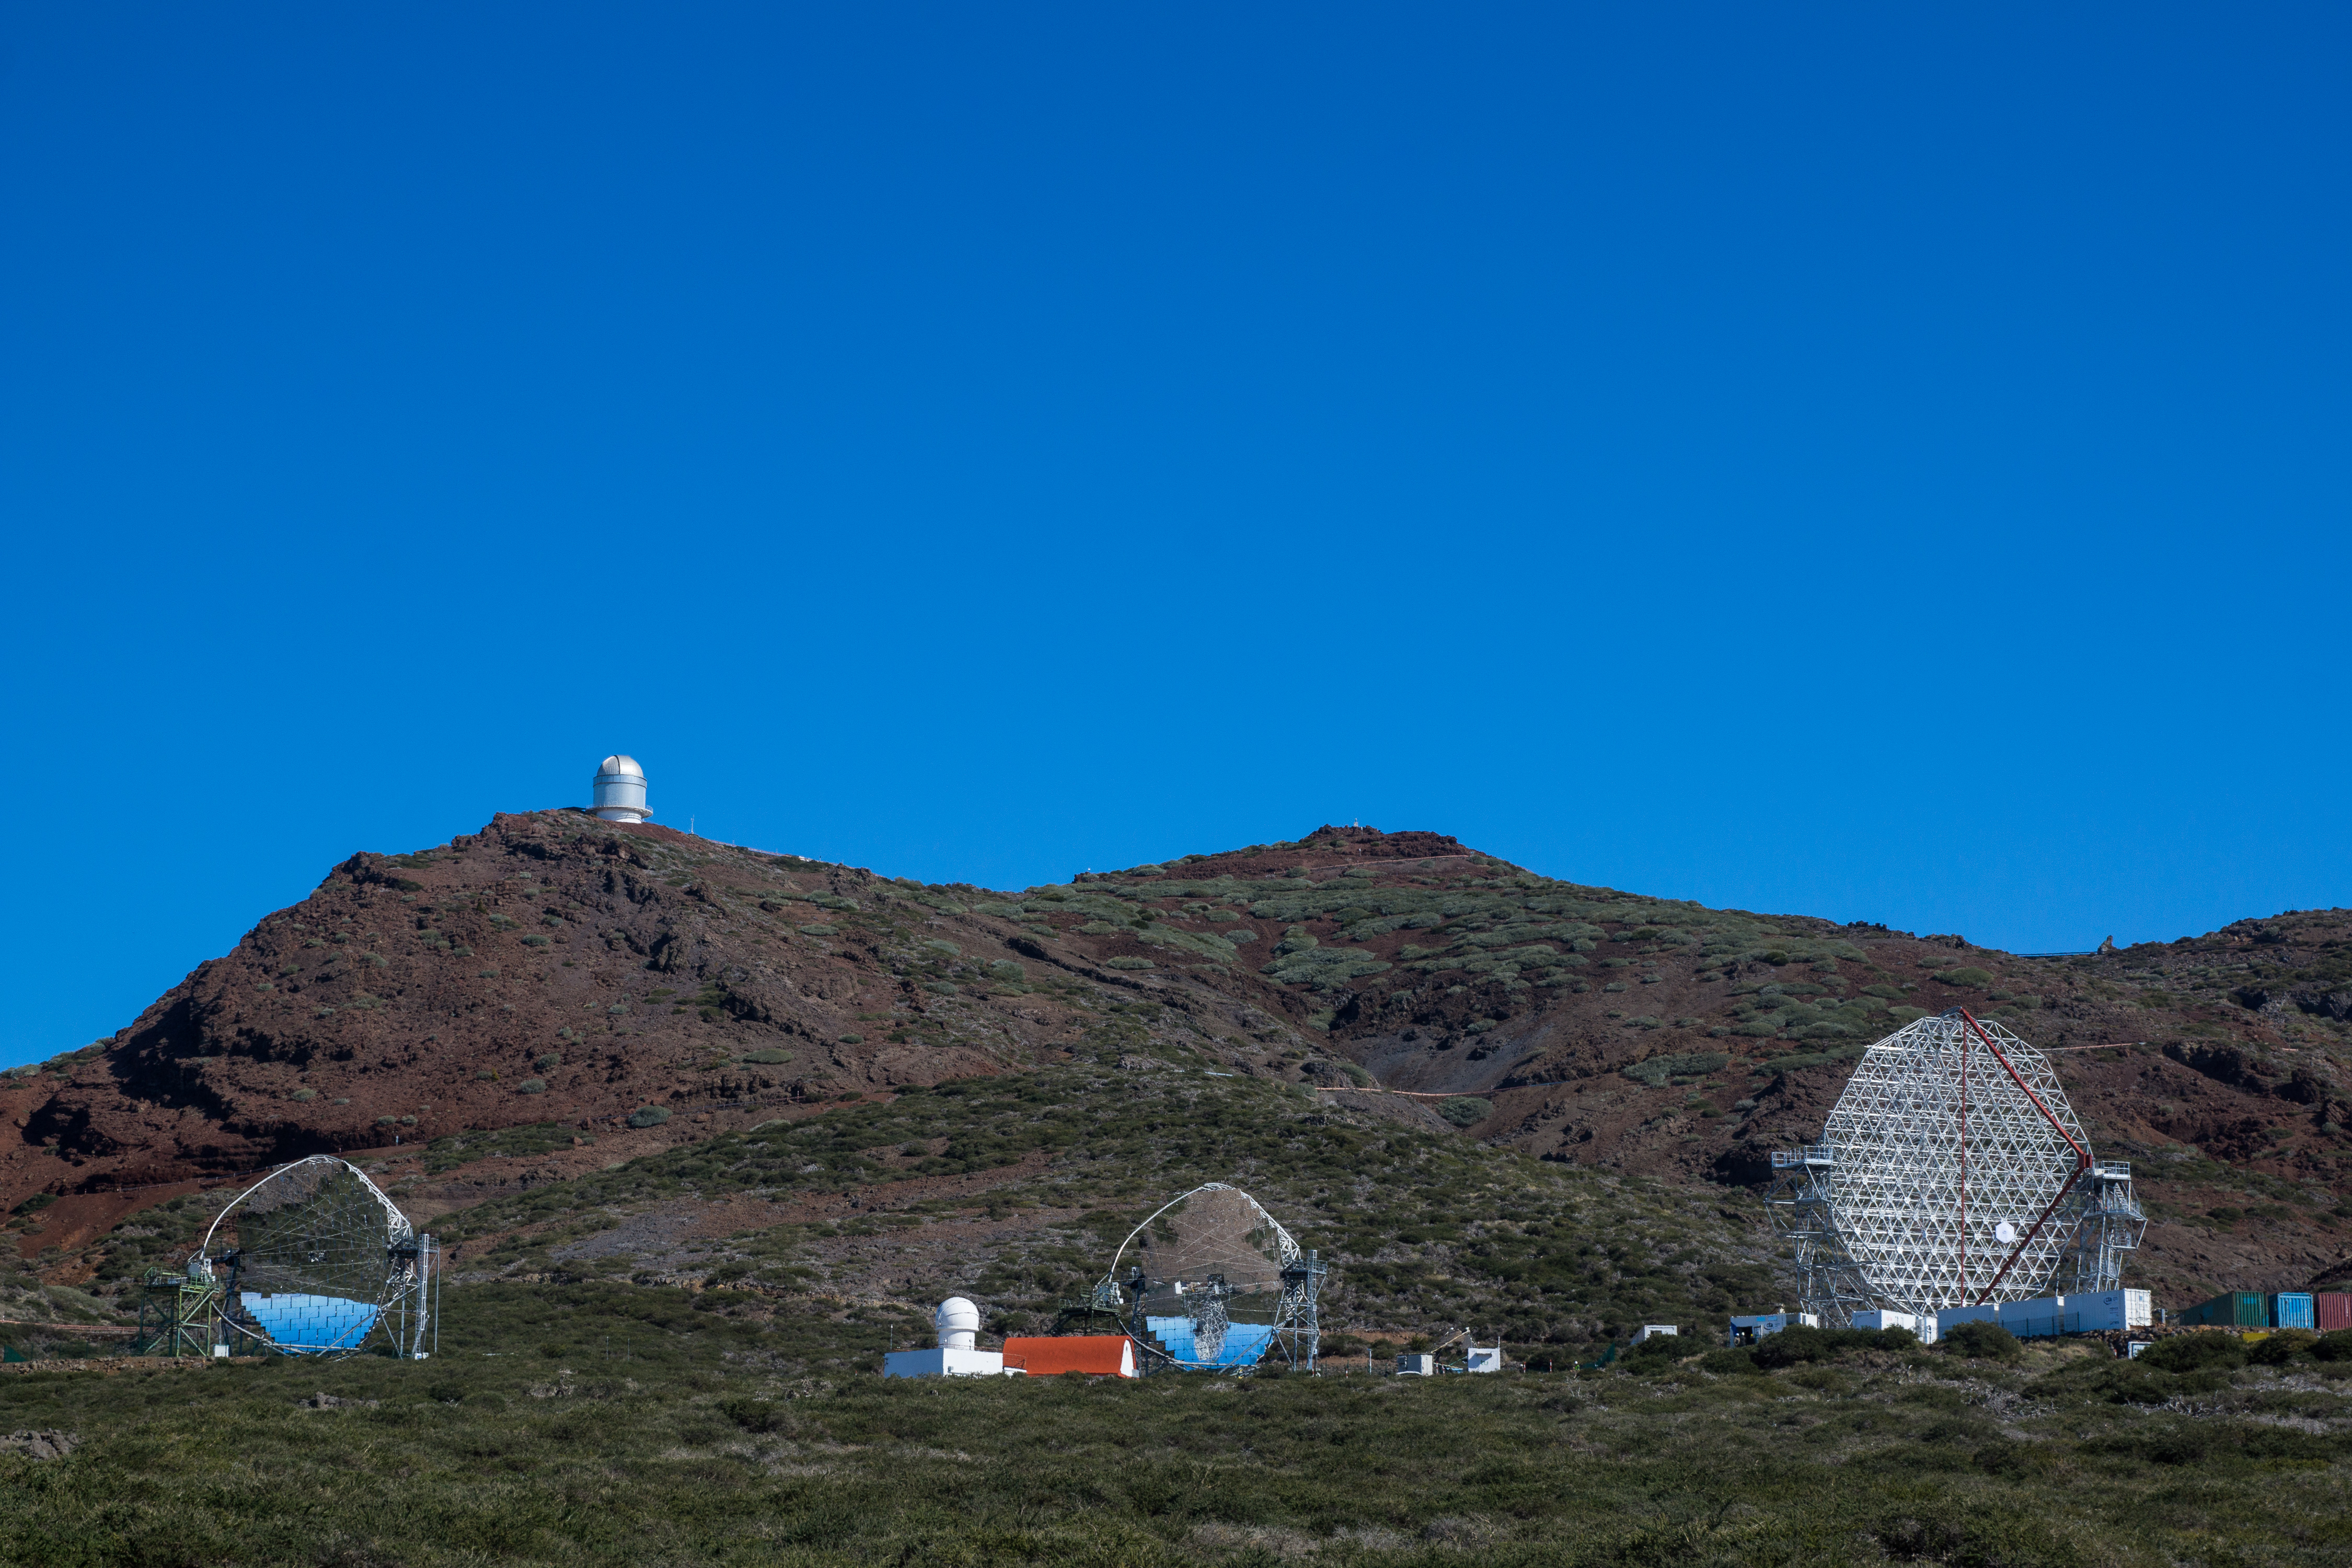
\includegraphics[width=\linewidth, trim={0 3cm 0 12cm}, clip]{images/magic_fact_lst.jpg}
  \caption{%
    The \gls{magic}, \gls{fact} and LST-1 telescopes (from left to right) at the \gls{orm} in April 2018,
    when the LST-1 was still under construction.
  }\label{fig:orm}
\end{figure}

To improve upon the sensitivity of the currently operating telescopes by at least 
an order of magnitude, both in the northern and the southern hemisphere, 
a large international consortium is currently planning and building the \gls{cta}.
In its final form, it will comprise 99 telescopes at the southern observatory in
Chile and 19 telescopes at the northern site at the \gls{orm}~\cite{science-cta}.
As of November 2019, prototypes for all of the three different telescope sizes
are developed and the first \SI{23}{\meter} Large Sized Telescope is in commissioning
at La~Palma and detected its first signal of the Crab Nebula~\cite{lst-crab}.
Construction of the full array will take several years and is currently planned
to be finished in 2025~\cite{cta-status}.

As one major open question is the variability of \glspl{agn}, see \autoref{sec:agn},
dense, unbiased\footnote{The currently observing large telescopes tend only to observe
\gls{agn} in active states when triggered through an external alert, thus having a
large selection bias on possible flux states.} monitoring of these objects is crucial to understand the underlying processes.
A possible solution for this would be to install Cherenkov telescopes around the globe
at multiple locations so that at least one telescope can observe a source at
any given time.
\gls{fact} was started as a prototype for a telescope in such a ring, but 
having larger telescopes with higher sensitivity for the short scale variability
would improve the possible scientific results dramatically~\cite{ctr}.

\subsection{Water Cherenkov Telescopes}

The third possibility of detecting high energy gamma-radiation is
measuring the energetic particles produced in air showers that reach the ground
using water Cherenkov tanks.
These large volume tanks contain photosensors that detect the Cherenkov light
produced by particles going through the water.
As these water tanks are closed, these observatories are not bound to observing
only in dark nights and are much less affected by weather conditions in comparison
to \glspl{iact}.
Also, they observe the whole sky above them at any given time, though 
sensitivity is limited beyond zenith distances of more than \ang{45}.
The only currently operating observatory using this detection mechanism is
the \gls{hawc} experiment in Mexico~\cite{hawc-monitoring}.
\gls{hawc} is fully operational using 300 water tanks with \SI{190}{\cubic\meter}
of water each since 2015, each tank is outfitted with four \glspl{pmt}~\cite{hawc-monitoring}.
\gls{hawc}'s sensitivity for point sources is lower than for most \glspl{iact} in the
common energy range, but it can monitor many sources at the same time.


\section{Sources of Gamma Radiation}\label{sec:sources}
\begin{figure}
  \centering
  \includegraphics{build/plots/4fgl_fact_sources.pdf}
  \caption{%
    The gamma-ray sky as observed by the Large Area Telescope aboard the 
    \textit{Fermi}-Satellite in equatorial coordinates and equal-area Mollweide projection.
    The color of the points indicates particle flux between \SI{1}{\GeV} and \SI{100}{\GeV}.
    A gray band shows the galactic plane.
    The seven sources most observed by \gls{fact} are marked. 
    All but the Crab Nebula, which is a \gls{snr}, are blazars.
    Data taken from the 4FGL~\cite{4fgl}.
  }\label{fig:4fgl}
\end{figure}
\noindent High energy gamma radiation can originate from two main source types.
Gamma rays from inside the Milky Way are mostly produced in super nova remnants,
mostly pulsars, \gls{pwn} and shell-type super novae.
Extragalactic sources are dominated by \glspl{agn}, the very bright central regions of galaxies containing super massive black holes with \num{e6} to \num{e10} solar masses $M_\odot$~\cite{app-angelis}.

\subsection{Active Galactic Nuclei}\label{sec:agn}
Outside of our own galaxy, the most numerous, lasting sources
of gamma radiation are \glspl{agn}, galaxies with super massive black holes at their centers.
These black holes accrete matter from the surrounding medium,
forming disks around the black hole.
These objects belong to the brightest in the universe, reaching powers
of \SI{e40}{\watt}~\cite{app-angelis}.
In some cases, narrow, relativistic jets of particles shoot out perpendicular to the accretion disk of matter falling into the black hole.
\begin{wrapfigure}[23]{O}{0.5\textwidth}
  \includegraphics[width=\linewidth]{images/m87.jpg}
  \caption{%
    Hubble image of the radio galaxy M87, an \gls{agn} with
    a larger viewing angle than blazars, so the relativistic jet is visible.~\cite{hubble-m87}.
    The central black hole of M87 was also the first to be directly imaged through
    \gls{vlbi}~\cite{m87-bh}.
  }\label{fig:m87}
\end{wrapfigure}

The jet producing \glspl{agn} are classified into categories based on the viewing angle
towards the jet.
A viewing direction nearly down the jet and the resulting Doppler-boosting classify an \gls{agn} as blazar
and these are the main sources of high energy, extra-galactic gamma rays.
Blazars are subdivided into two categories based on the existence
or absence of line emission in the optical spectrum.
\glspl{fsrq} show broad line emissions, likely from gas clouds closely orbiting the black hole, and generally have a higher energy output than
BL Lacertae objects, named after the prototypical source, 
that show no or very weak line emissions~\cite{fromblazars}.

While BL Lac objects have lower overall energy output, they reach
higher energies and are the predominant extra-galactic source type
at \si{\TeV} energies.
The 4FGL catalog contains 1109 BL Lac objects, 652 \glspl{fsrq} and 1310 blazars of
uncertain type~\cite{4fgl}.
Compared to that, TeVCat~\cite{tevcat},
an online catalog keeping track of gamma-ray observations at \si{\TeV} energies,
lists 52 BL Lac objects and only 6 \glspl{fsrq} to be detected in this energy range.

The gamma-ray flux of blazars is characterized over more than ten magnitudes
by a double hump structure. 
The first, low energy hump is universally assumed to be from synchroton radiation
of high energy electrons and peaks in the infrared to soft X-ray band.
The second, high energy hump is not fully understood and two main classes 
of models try to describe the high energy emission, either
purely leptonic models or models including hadronic components.

The simplest model describing gamma-ray flux from blazars is the single zone,
synchroton self-Compton model.
Assuming a single population of high energy electrons, low energy photons
are created by synchroton radiation and some of these photons gain energy
from the same population of electrons via inverse Compton scattering.
This scenario is purely leptonic and would not require high energy protons,
thus excluding these sources as possible origin of high energy cosmic rays.

However, some blazars show hints of a hadronic component, where additional
high energy photons are created by neutral pion decays~\cite{fromblazars}. 
As these hadronic reactions would also produce charged pions, which in turn
decay into neutrinos, observations of neutrinos from blazars would be the \enquote{smoking gun}
for blazars being sources of high energy cosmic rays.
A first strong hint for neutrinos from a blazar was published in 2018 by the
IceCube collaboration, where first a single, 
high energy neutrino from a direction consistent with the blazar TXS0506+056 
simultaneously with a flare in the electromagnetic spectrum of the source was observed~\cite{txs}.
In a second step, IceCube found an excess of lower energy neutrinos from the direction
of the source in historic data with a significance of \SI{3.5}{\sigma}~\cite{txs-historic}.

Blazars show large variability of their flux states,
both on long time scales slowly changing their mean power over months and years
and on very short time scales, doubling their flux in mere minutes, 
contesting the more simple models for blazar emission that cannot describe 
variability on such short timescales~\cite{fromblazars}.
In a very bright outburst in 2005, \gls{magic} observed a doubling of the flux of Mrk~501
in only two minutes~\cite{mrk501-variability}.

\subsection{Super Nova Remnants}
Most individual sources of gamma radiation in our own galaxy are the different types
of super nova remnants~\cite{tevcat, 4fgl}, what is left behind by the violent
death of a massive star.
Depending on the mass of the progenitor star and the age of the \gls{snr}, 
three related main classes exist: pulsars, \glspl{pwn} and shell-type \glspl{snr}.

% \begin{wrapfigure}[25]{O}{0.4\textwidth}
%   \includegraphics[width=\linewidth]{images/crab.jpg}
%   \caption{%
%     Multi-wavelength image of the Crab Nebula in pseudo-colors.
%     Observations of five different telescopes were combined:
%     VLA (radio, red), Spitzer Space Telescope (infrared, yellow), Hubble Space Telescope (visible, green),  XMM-Newton (ultraviolet, blue) and Chandra X-ray Observatory (purple)~\cite{crab-mwl}.
%     The central part dominated the purple X-ray observations shows the pulsar with its accretion disk and jet.
%   }\label{fig:crab}
% \end{wrapfigure}

\begin{figure}
  \begin{captionbeside}{
    Multi-wavelength image of the Crab Nebula in pseudo-colors.
    Observations of five different telescopes were combined:
    VLA (radio, red), Spitzer Space Telescope (infrared, yellow), Hubble Space Telescope (visible, green),  XMM-Newton (ultraviolet, blue) and Chandra X-ray Observatory (purple)~\cite{crab-mwl}.
    The central part, dominated by the purple X-ray observations, shows the pulsar with its accretion disk and jet.
  }%
    \small%
    \raisebox{\dimexpr\baselineskip-\totalheight\relax}{%
      \includegraphics[width=0.5\linewidth]{images/crab.jpg}
    }% 
  \end{captionbeside}\label{fig:crab}
\end{figure}

Stars are in an equilibrium between gravitational force trying to
collapse them and radiative pressure preventing this.
After a star burned through most of its hydrogen fuel,
the radiative pressure falls and the star starts to collapse until three helium nuclei can be fused 
into carbon and pressure is built up again keeping the star stable once more, now
burning through its helium supply.
This repeats several times—each time producing heavier elements—until iron is reached,
which is the last element where fusion produces energy.
If the remaining core is more massive than $\num{1.4} M_\odot$, the core collapses
into a neutron star, if the mass is larger than 3 to 5 times $M_\odot$, it will collapse 
into a black hole.
The collapse also results in the supernova explosion.~\cite{app-angelis}

Neutron stars are only \SIrange{10}{20}{\kilo\meter} in diameter and
rotate very quickly, because of the conservation of angular momentum
and show extreme magnetic fields up to \SI{e8}{\tesla}~\cite{app-angelis}.
If the rotation axis is not aligned with the magnetic field axis,
neutron stars are observed to emit pulsed beams of radiation,
These pulsars, found in most young \gls{snr},
are the most numerous galactic source type in the 4FGL catalog~\cite{4fgl}.
A pulsar can power gamma-ray emission in the surrounding gas cloud left over
from the supernova explosion, creating a \gls{pwn}.
The most prominent source of high energy gamma radiation, the Crab Nebula,
is a \gls{pwn} created by a supernova explosion in 1054, observed by Chinese
and Japanese astronomers, visible at daylight for 23 days~\cite{sn1054}.
A pseudo-color image of the Crab Nebula from multiple observatories is shown in \autoref{fig:crab}.

Particle acceleration happens very similar to the mechanisms proposed for \gls{agn}
and the Crab Nebula is particularly well described via a purely leptonic 
synchroton and inverse Compton model,
using two different electron spectra and four photon distributions: 
the synchroton radiation (the self Compton part), thermal emissions from dust, the
cosmic microwave background and line emission from the nebula~\cite{meyer-crab}.
The full spectral energy distribution from the radio regime to very high energy
gamma radiation as measured by several experiments is shown in \autoref{fig:crab-sed}.
The Crab Nebula also shows a rather constant flux at very high energies and
has thus become the \enquote{standard candle} of VHE gamma-ray astronomy~\cite{meyer-crab}.
The Crab Nebula is used as reference for sensitivities, also in this work, and
as a unit of flux: \SI{1}{CU} being the flux of the Crab Nebula either differential
at a certain energy or integrated over a specific energy range.
The \gls{magic} collaboration published a log-parabola parameterization of
the Crab Nebula flux  valid for the whole energy range observable by \gls{fact} in \cite{magic-crab}:
\begin{equation}
  \Phi(E) = \frac{\num{3.23e-11}}{\si{\TeV\cm\squared\second}}
  \left(\frac{E}{\SI{1}{\TeV}}\right)^{\num{-2.47} - \num{0.24} \log_{10}(\sfrac{E}{\SI{1}{\TeV}})}. \label{eq:magic-crab}
\end{equation}
This parameterization will be used as reference spectrum to calculate the weights
for simulated events in \autoref{chp:performance}.

\begin{landscape}%
  \sisetup{per-mode=reciprocal}%
  \input{build/plots/crab_sed.pgf}\\
  \captionof{figure}{%
    Spectral energy distribution of the Crab Nebula, data from 16 observatories,
    available in a single data file from \cite{gammapy-crab}. 
    The gray line shows the parameterization of the inverse Compton part of the spectrum
    from \cite{meyer-crab}.
  }\label{fig:crab-sed}%
  \sisetup{per-mode=symbol-or-fraction}%
\end{landscape}

\subsection{Gamma-Ray Bursts}

The third class of gamma-ray sources are the short, transient bursts of gamma radiation
which are also of extra-galactic origin.
Two classes of bursts exist, bursts with durations longer than two seconds are
currently thought to be caused by core-collapse super novae, they make up around \SI{70}{\percent}
of the detected bursts.
One source for the bursts shorter than two seconds was confirmed in 2017, 
when LIGO and VIRGO observed a gravitational wave event caused by the merger of two 
neutron stars and a \gls{grb} was detected \SI{1.7}{\second} after this signal by the \textit{Fermi} satellite. 
Later, the kilonova was observed and detected by 70 observatories all around the globe
and in Earth's orbit. 
This first event measured both electromagnetically and in gravitational waves
was named \enquote{Science Breakthrough of the Year 2017}~\cite{neutron-star-merger}
and was the first true multi-messenger observation.

\section{Key Science Questions}\label{sec:science}

Stefan Funk~\cite{funk-gamma} and the \gls{cta} Consortium~\cite{science-cta} identify the following
questions as most relevant to currently observing and planned gamma-ray observatories:

\paragraph{The Origin of Charged Cosmic Rays}
Since first discovered by Victor F. Hess in 1912~\cite{hess1912},
the origin of the charged cosmic rays remain largely unknown.
Several candidates have been proposed, but none identified with certainty.
If gamma-ray sources would be discovered to show spectra only explainable 
using hadronic models, this would offer a strong hint that those sources also produce
charged cosmic rays.
This can only be an indirect proof compared to neutrino observations,
which would directly point to hadronic reactions.

\paragraph{The Search for Dark Matter}
High energy gamma-ray astronomy is sensitive to annihilation lines
created by several proposed candidates for dark matter particles,
e.\,g.\ by two \glspl{wimp} converting into two gamma rays.
Also theories for axion-like particles will be tested via the proposed changes to the
mechanics of the \gls{ebl} absorption.

\paragraph{Understanding Acceleration Mechanisms}
The precise mechanisms at work in the extreme environments of
\gls{agn} and pulsars are still a largely open question, 
especially the very short time scale variability is not described by current models.

\paragraph{Cosmology and Fundamental Physics}
\glspl{iact} are able to test a number of predictions made by 
several theories of quantum gravity, e.\,g.\ Lorentz invariance violations.
This is also connected to the question of dark matter.

\section{Cosmic Rays}\label{sec:cosmic-rays}
Charged primary particles are the main background class for any
gamma-ray telescope, also for \glspl{iact}.
As they are deflected by magnetic fields in the interstellar and
intergalactic medium, their origin is not reconstructible at rigidities 
relevant to \glspl{iact} and they thus form an isotropic, diffuse background.
\begin{figure}
  \centering
  \includegraphics{build/plots/proton_helium_spectrum.pdf}
  \caption{%
    Particle flux of protons (solid colors) and
    helium nuclei (transparent) as measured by several experiments.
    Data from \cite{cr-database}.
    The two gray lines are the respective fit results shown in \eqref{eq:proton-flux} and
    \eqref{eq:helium-flux}.
  }\label{fig:cr-flux}
\end{figure}

\autoref{fig:cr-flux} shows the flux of primary protons and helium nuclei between
\SI{1}{\GeV} and \SI{1}{\peta\eV}. 
These two elements make up over \SI{90}{\percent} of the charged cosmic rays
around \SI{1}{\GeV}~\cite{pdg}. 
At the energies relevant for \gls{fact}, above \textasciitilde\SI{100}{\GeV},
helium nuclei are almost as abundant as protons.
The flux of all charged primaries can be approximated above $\approx \SI{100}{\GeV}$
using
\begin{equation}
  I_N(E_N) \approx
  \frac{\num{1.8e4}}{\si{\GeV\meter\squared\second\steradian}}
  \left(\frac{E_N}{\SI{1}{\GeV}}\right)^{\num{-2.7}}
  \quad \text{\cite[(29.2)]{pdg}} \label{eq:all-particle}
\end{equation}
where $E_N$ is the energy \emph{per nucleon}.

The individual spectra for proton and helium nuclei are described using power laws
obtained by linear regression of $\log_{10}(I)$ vs. $\log_{10}(E)$ using
the data shown in \autoref{fig:cr-flux}.
For the proton flux, this yields
\begin{equation}
  I_\text{p}(E) = \frac{\input{build/proton_norm.tex}}{\si{\GeV\meter\squared\second\steradian}}
  \left(\frac{E}{\SI{1}{\GeV}}\right)^{\input{build/proton_index.tex}}
  \label{eq:proton-flux}
\end{equation}
and for the helium flux per nucleus, \emph{not nucleon},
\begin{equation}
  I_\text{He}(E) = \frac{\input{build/helium_norm.tex}}{\si{\GeV\meter\squared\second\steradian}}
  \left(\frac{E}{\SI{1}{\GeV}}\right)^{\input{build/helium_index.tex}}
  \label{eq:helium-flux}
\end{equation}
is obtained.
The covariance matrices for the fits are given in Appendix~\ref{apx:fit-results}.


For an observation of the Crab Nebula, the ratio
of gamma rays from the source to cosmic ray background events will approximately be
\begin{align}
  \frac{N_\gamma}{N_\text{CR}} &=
  \frac%
  {\int_{\Emin}^{\Emax} \int_A \int_{t_0}^{t_1} \Phi(E) \d{t} \d{A} \d{E}}%
  {\int_{\Emin}^{\Emax} \int_A \int_\Omega \int_{t_0}^{t_1} I_N(E) \d{t} \d{\Omega} \d{A} \d{E}}\\
  \intertext{%
    where $\Phi$ is the flux of the Crab Nebula, which for most \glspl{iact} can
    be assumed to be a point source and thus no integration over the solid angle is necessary.
    We can now calculate this ratio for an \gls{iact} with a field of view with a diameter
    of \SI{4.5}{\degree}, resulting in $\Omega = 2\PI (1 - \cos{\SI{2.25}{\degree}})\, \si{sr} \approx \SI{0.005}{\steradian}$. 
    The area of the detector and the observation time is the same for both terms and
    cancels out.
  }%
  \frac{N_\gamma}{N_\text{CR}} &= \frac%
  {\int_{\Emin}^{\Emax} \Phi(E) \d{E}}%
  {\SI{0.005}{\steradian} \int_{\Emin}^{\Emax} I_N(E) \d{E}}
  \intertext{using the log-parabola parameterization of the Crab Nebula flux published by
  the \gls{magic} collaboration in \cite{magic-crab} and an energy range of \SI{100}{GeV}
  to \SI{200}{\TeV} results in}
  \frac{N_\gamma}{N_\text{CR}} &\approx \frac{1}{4300}
\end{align}

So for each gamma-ray induced shower, 4300 showers induced by charged cosmic rays
are reaching the telescope.
We will see in \autoref{sec:sensitivity} that \gls{fact} can detect sources with down to \SI{10}{\percent} 
of the flux of the Crab Nebula in \SI{50}{\hour} of observation time, 
\gls{magic} is an order of magnitude more sensitive reaching around one percent
in \SI{50}{\hour} \cite{magic-performance}.
This directly translates into the ratio of signal to background events and
will necessitate an analysis that can classify recorded events as either 
gamma-ray or cosmic-ray induced to suppress this background as much as possible.
Methods to achieve this will be introduced in \autoref{chp:reconstruction}.
